Conclusa la presentazione delle scelte adottate in fase di impostazione delle sperimentazioni, 
si procede in questo capitolo con l'esposizione dei risultati ottenuti. 

Per effettuare la risoluzione delle diverse istanze, è stato utilizzato un cluster messo a disposizione dal Dipartimeto di Ingegneria dell'Informazione 
dell'università. Nello specifico, la macchina in questione presenta le seguenti specifiche tecniche:
\begin{itemize}
\item Intel(R) Xeon(R) CPU E5-2623 v3 @ 3.00GHz quad-core
\item 16GB RAM
\item Linux Fedora 37
\item Python 3.10.6
\item IBM ILOG CPLEX Optimization Studio versione 22.1
\end{itemize}
Per garantire la compatibilità tra l'ultima versione del software CPLEX installata (22.1) e quella di Python, è stato fatto uso di \textit{pyenv} \cite{pyenv}, 
un'utility per Linux e MacOS che permette di tenere all'interno dello stesso sistema operativo differenti versioni dell'interprete Python. In questo modo 
è stato possibile utilizzare la versione Python richiesta da CPLEX (3.10) e non quella predefita del cluster (3.11).

Inoltre, sono state installate localmente tutte le librerie che vengono utilizzate all'interno dei vari script, che si ricordano 
essere: \textit{Numpy}, \textit{Pyomo}, \textit{Matplotlib} e \textit{Seaborn}.

\newpage
\section{Tempi medi di risoluzione}
I tempi medi, estrapolati e memorizzati come illustrato nelle sezioni precedenti, sono riportati nelle seguenti tabelle indicizzate sulla dimensione delle istanze 
e sui valori di densità di grigio utilizzati.per generare quest'ultime.

I tempi sono riportati nel formato \textit{hh:mm:ss.00}, dove \textit{hh} indica il numero di ore impiegate, \textit{mm} i minuti e \textit{ss.00} i secondi arrotondati 
alla seconda cifra dopo la virgola. \\

\begin{tabular}{cc c|c|c|c l}
    \centering
    & & \multicolumn{3}{ c }{Dimensione dell'istanza \textit{n}} \\ \cline{3-5}
    & & \multicolumn{1}{ |c| }{9 (3x3)} & 16 (4x4) & 25 (5x5) & \\ \cline{2-5}
    \multicolumn{1}{  c  }{\multirow{8}{*}{Densità di} } &
    \multicolumn{1}{ |c| }{10\%} & 00:00:00.17 & 00:00:00.12 & 00:00:00.28 &   \\ \cline{2-5}
    \multicolumn{1}{  c  }{}                        &
    \multicolumn{1}{ |c| }{20\%} & 00:00:00.14 & 00:00:00.10 & 00:00:00.27 &    \\ \cline{2-5}
    \multicolumn{1}{  c  }{}                        &
    \multicolumn{1}{ |c| }{30\%} & 00:00:00.05 & 00:00:00.12 & 00:00:00.34 &    \\ \cline{2-5}
    \multicolumn{1}{  c  }{}                        &
    \multicolumn{1}{ |c| }{40\%} & 00:00:00.04 & 00:00:00.21 & 00:00:01.59 &    \\ \cline{2-5}
    \multicolumn{1}{  c  }{\multirow{1}{*}{grigio \textit{d}}}                        &
    \multicolumn{1}{ |c| }{50\%} & 00:00:00.04 & 00:00:00.23 & 00:00:02.59 &    \\ \cline{2-5}
    \multicolumn{1}{  c  }{}                        &
    \multicolumn{1}{ |c| }{60\%} & 00:00:00.06 & 00:00:00.22 & 00:00:02.46 &    \\ \cline{2-5}
    \multicolumn{1}{  c  }{}                        &
    \multicolumn{1}{ |c| }{70\%} & 00:00:00.05 & 00:00:00.13 & 00:00:00.68 &    \\ \cline{2-5}
    \multicolumn{1}{  c  }{}                        &
    \multicolumn{1}{ |c| }{80\%} & 00:00:00.05 & 00:00:00.12 & 00:00:00.48 &    \\ \cline{2-5}
    \multicolumn{1}{  c  }{}                        &
    \multicolumn{1}{ |c| }{90\%} & 00:00:00.03 & 00:00:00.13 & 00:00:00.32 &    \\ \cline{2-5}
    \medskip
\end{tabular}

\begin{tabular}{cc c|c|c|c l}
    & & \multicolumn{3}{ c }{Dimensione dell'istanza \textit{n}} \\ \cline{3-5}
    & & \multicolumn{1}{ |c| }{36 (6x6)} & 42 (7x6) & 45 (9x5) & \\ \cline{2-5}
    \multicolumn{1}{  c  }{\multirow{8}{*}{Densità di} } &
    \multicolumn{1}{ |c| }{10\%} & 00:00:00.59 & 00:00:00.84 & 00:00:01.08 &   \\ \cline{2-5}
    \multicolumn{1}{  c  }{}                        &
    \multicolumn{1}{ |c| }{20\%} & 00:00:00.85 & 00:00:05.03 & 00:00:12.99 &    \\ \cline{2-5}
    \multicolumn{1}{  c  }{}                        &
    \multicolumn{1}{ |c| }{30\%} & 00:00:13.00 & 00:04:56.35 & 00:15:13.03 &    \\ \cline{2-5}
    \multicolumn{1}{  c  }{}                        &
    \multicolumn{1}{ |c| }{40\%} & 00:01:06.86 & 00:26:51.01 & 01:21:36.74 &    \\ \cline{2-5}
    \multicolumn{1}{  c  }{\multirow{1}{*}{grigio \textit{d}}}                        &
    \multicolumn{1}{ |c| }{50\%} & 00:00:18.40 & 00:06:13.01 & 00:49:02.35 &    \\ \cline{2-5}
    \multicolumn{1}{  c  }{}                        &
    \multicolumn{1}{ |c| }{60\%} & 00:01:37.72 & 00:36:49.48 & 01:51:47.95 &    \\ \cline{2-5}
    \multicolumn{1}{  c  }{}                        &
    \multicolumn{1}{ |c| }{70\%} & 00:01:10.83 & 00:27:21.45 & 01:37:33.22 &    \\ \cline{2-5}
    \multicolumn{1}{  c  }{}                        &
    \multicolumn{1}{ |c| }{80\%} & 00:00:06.37 & 00:00:36.44 & 00:02:38.68 &    \\ \cline{2-5}
    \multicolumn{1}{  c  }{}                        &
    \multicolumn{1}{ |c| }{90\%} & 00:00:00.77 & 00:00:01.30 & 00:00:05.66 &    \\ \cline{2-5}
\end{tabular}

\newpage \noindent
Tramite uno script \textit{Python} che fa uso di alcuni comandi delle librerie \textit{NumPy} e \textit{Matplotlib}, questi dati 
sono stati utilizzati per creare un grafico 3D ed uno 2D. Tali grafici sono stati realizzati per permettere di comprendere al meglio i risultati 
degli esperimenti ottenuti e di notare facilmente qual'è l'andamento del tempo di risoluzione delle istanze rispetto ai valori assunti dai 
parametri di generazione \textit{n} e \textit{d}.
\begin{figure}[h!]
    \centering
    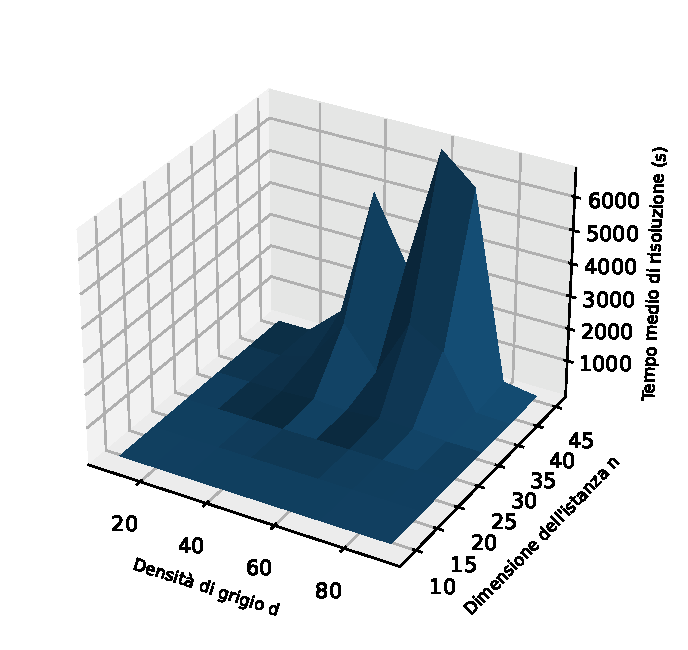
\includegraphics[scale=0.9]{images/resolution_times.eps}
    \caption{Grafico 3D dei tempi di risoluzione delle istanze Tai*c testate}
    \label{fig:times}
\end{figure}
\begin{figure}[h!]
    \centering
    \includegraphics[scale=0.59]{images/resolution_times2.eps}
    \caption{Grafico 2D dei tempi di risoluzione delle istanze Tai*c testate}
    \label{fig:times2}
\end{figure}

Come si evince dai grafici, il comportamento assunto dei tempi di risoluzione rispetto alla dimensione dell'istanza è generalmente 
esponenziale, indipendentemente dal valore di densità di grigio considerato. Ciò che muta da una curva dei tempi rispetto all'altra è la 
velocità con cui i valori divergono. Nello specifico si nota come la crescita dei tempi per le densità intermedie $40\%$, $60\%$ e $70\%$ 
è maggiore rispetto a quella per $d=50\%$, che a sua volta è notevolmente maggiore rispetto a quella per le densità $10\%$ e $90\%$.

È possibile dunque affermare che a parità di dimensione \textit{n}, le istanze Tai*c che richiedono un maggior tempo 
di risoluzione sono quelle generate da un valore di densità di grigio \textit{d} prossimo, ma non corrispondente, al $50\%$, mentre quelle 
che ne richiedono meno sono quelle generate da valori di \textit{d} prossimi allo $0\%$ o al $100\%$.

Questo risultato corrisponde con quello ipotizzabile limitandosi ad osservare la teoria. Infatti, per densità prossime allo $0\%$ il numero 
di unità da assegnare alle posizioni è ridotto ed invece per densità prossime al $100\%$, il numero di posizioni in cui non deve essere asseganta un'unità 
è esiguo. Per questo motivo si suppone che in ambo i casi il costo computazionale richiesto per trovare la soluzione ottima sia ridotto. 
Diversamente accade per densità vicine al $50\%$, valore per il quale il numero di posizioni essegnate ad un'unità è simile a quello delle 
posizioni libere. È pertanto comprensibile che si abbia il picco di complessità per tali valori.

La dimensione $45\,(9\times 5)$ è stata l'ultima per la quale è stato possibile ricavare, al time limit di 2 ore, un tempo di risoluzione medio per 
ogni valore di densità di grigio. Difatti, per le istanze di dimensione $49\,(7\times 7)$ sono stati ottenuti i seguenti dati:

\begin{tabular}{cc c|c|c|c|c| l}
    & & \multicolumn{5}{ c }{Densità di grigio \textit{d}} \\ \cline{3-7}
    & & \multicolumn{1}{ |c| }{10\%} & 20\% & 30\% & 40\% & 50\% &  \\ \cline{2-7}
    \multicolumn{1}{  c  }{\multirow{1}{*}{\textit{n}}}  &
    \multicolumn{1}{ |c| }{49(7x7)} & 00:00:01.19 & 00:00:43.57 & 00:51:50.19 & 12.04\% & 1.17\% \\ \cline{2-7}
\end{tabular}

\begin{tabular}{cc c|c|c|c| l}
    & & \multicolumn{4}{ c }{Densità di grigio \textit{d}} \\ \cline{3-6}
    & & \multicolumn{1}{ |c| }{60\%} & 70\% & 80\% & 90\% & \\ \cline{2-6}
    \multicolumn{1}{  c  }{\multirow{1}{*}{\textit{n}}}  &
    \multicolumn{1}{ |c| }{49(7x7)} & 6.39\% & 3.02\% & 00:17:24.36 & 00:00:08.39 \\ \cline{2-6}
    \medskip
\end{tabular}

In queste tabelle compaiono valori di tipo diverso. Dato un valore di densità \textit{d}, se nella relativa cella compare un tempo, esso corrisponde al tempo medio di esecuzione per \textit{d}, mentre dove 
compare una percentuale significa che per quel \textit{d} non è stato possibile calcolare il tempo cercato e pertanto è stato riportato il valore dell'\textit{optimality gap} al \textit{time limit} impostato di due ore.


\newpage
\section{Soluzioni trovate}